\documentclass{article}
\usepackage{amsmath}
\usepackage{graphicx}

\begin{document}

\title{An Expedition to The Valley of Genomics}
\author{Your Name}
\date{\today}

\maketitle



\section{29-05-2023}
\subsection{Commits}
\paragraph{Commit: bd81b50}
Commit Message: Hoy hicimos un workflow en el que cada commit se va guardado en el diario de laboratorio, con su id y con su mensaje. También se genera una sección de figuras para las figuras que fueron generadas en esa sesión

\paragraph{Commit: 7997396}
Commit Message: pruebo figura

\paragraph{Commit: 50ff4b4}
Commit Message: pruebo figura

\paragraph{Commit: 459b400}
Commit Message: ol

\paragraph{Commit: 1d47914}
Commit Message: prueba

\paragraph{Commit: ba9ba18}
Commit Message: prueba

\paragraph{Commit: 6029931}
Commit Message: prueba

\paragraph{Commit: 2b666e3}
Commit Message: prueba

\paragraph{Commit: b987caa}
Commit Message: prueba

\paragraph{Commit: 39adf1f}
Commit Message: prueba

\paragraph{Commit: 2c3ca23}
Commit Message: prueba

\paragraph{Commit: dcf4e49}
Commit Message: prueba

\paragraph{Commit: fcdee47}
Commit Message: agrego la función parametro para probar las nuevas funciones

\paragraph{Commit: 435d42e}
Commit Message: en linear model lab agrego la capacidad de que la funcion model evaluating y la función calculate gene parameters puedan evaluar las nuevas métricas que se dispongan en la función parametro de phen_gen_weight_functions

\paragraph{Commit: 5b2b424}
Commit Message: agrego en el archivo plots.py la función accuracy para medir individualmente cada métrica

\paragraph{Commit: 99088c5}
Commit Message: modifico especificidad del gen poniendo k en logaritmo

\paragraph{Commit: d558a88}
Commit Message: arreglo la definición que había hecho de especificidad porque estaba mal escrita

\paragraph{Commit: e88a0b3}
Commit Message: prueba cambiando especificidad poniendo a k en un exponente de 10

\paragraph{Commit: cba1811}
Commit Message: arreglo algo que al parecer estaba mal en model_evaluating, que me confundí entre las variables n_metrica y nueva_muetrica, que son, dicho sea de paso, bastante inconvenientes los nombres, debería cambiar por otros

\paragraph{Commit: ff87169}
Commit Message: le saco los argumentos definidos de model evaluating y calculate gene parameters

\paragraph{Commit: 627b278}
Commit Message: ahora cambio True y False de nueva métrica por 'si' 'no', a ver si quizás es algo de eso

\paragraph{Commit: b43bb67}
Commit Message: también agrego una 'a' a un 'n_metric' que faltaba

\paragraph{Commit: 8eb196c}
Commit Message: cambio todos los betha por beta en linear model lab

\paragraph{Commit: 02318c3}
Commit Message: SOLUCIONADO. El problema estaba en calculate_gene_parameters, que asignabamos el booleano a nueva_metrica pero después esa variable cambiaba por el parámetro calculado para el gen candidato, ahora lo solucionamos y debería funcionar todo correctamente

\paragraph{Commit: 49694d7}
Commit Message: es decir que lo anterior no funcionaba no porque no calculase los parámetros sino porque no ordenaba el dataframe

\paragraph{Commit: eef3c10}
Commit Message: al parametro 3 de las nuevas métricas lo corrigo para no tener zerodivisionerror

\paragraph{Commit: e4d8092}
Commit Message: a especificidad_del_gen le agrego la feature type_of_func, para luego probar si queremos exponencial, logarítmica o lineal

%CommitsEnd
\subsection{Figures}

\begin{figure}[h] \centering 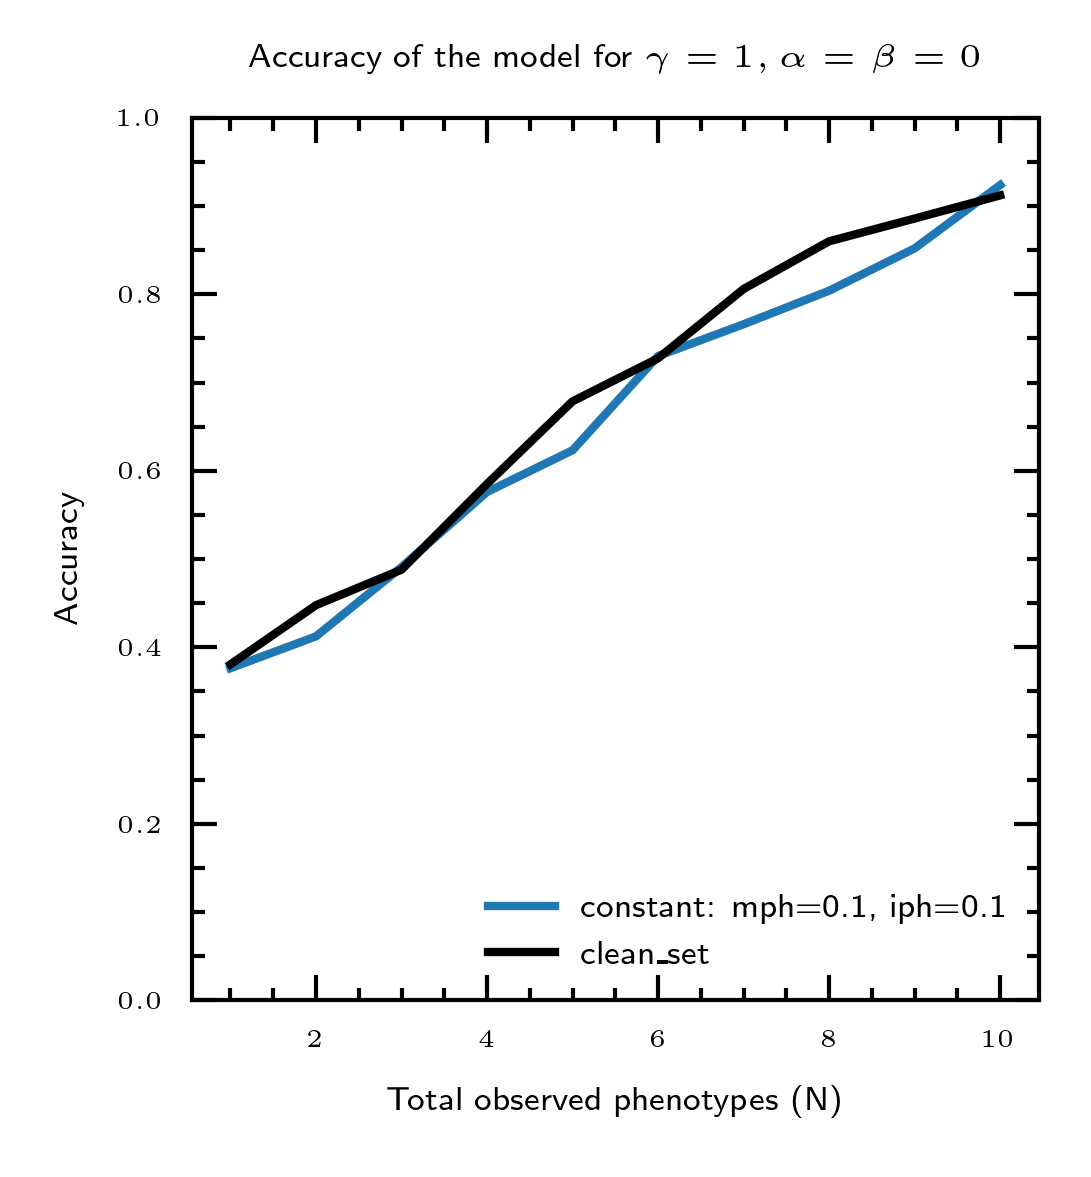
\includegraphics{n.png} \caption{Caption for n.png.} \end{figure}
%FiguresEnd
\subsection{Bibliography}
\subsection{Thoughts}

\section{04-06-2023}
\subsection{Commits}
\paragraph{Commit: fcdee47}
Commit Message: agrego la función parametro para probar las nuevas funciones

\paragraph{Commit: 435d42e}
Commit Message: en linear model lab agrego la capacidad de que la funcion model evaluating y la función calculate gene parameters puedan evaluar las nuevas métricas que se dispongan en la función parametro de phen_gen_weight_functions

\paragraph{Commit: 5b2b424}
Commit Message: agrego en el archivo plots.py la función accuracy para medir individualmente cada métrica

\paragraph{Commit: 99088c5}
Commit Message: modifico especificidad del gen poniendo k en logaritmo

\paragraph{Commit: d558a88}
Commit Message: arreglo la definición que había hecho de especificidad porque estaba mal escrita

\paragraph{Commit: e88a0b3}
Commit Message: prueba cambiando especificidad poniendo a k en un exponente de 10

\paragraph{Commit: cba1811}
Commit Message: arreglo algo que al parecer estaba mal en model_evaluating, que me confundí entre las variables n_metrica y nueva_muetrica, que son, dicho sea de paso, bastante inconvenientes los nombres, debería cambiar por otros

\paragraph{Commit: ff87169}
Commit Message: le saco los argumentos definidos de model evaluating y calculate gene parameters

\paragraph{Commit: 627b278}
Commit Message: ahora cambio True y False de nueva métrica por 'si' 'no', a ver si quizás es algo de eso

\paragraph{Commit: b43bb67}
Commit Message: también agrego una 'a' a un 'n_metric' que faltaba

\paragraph{Commit: 8eb196c}
Commit Message: cambio todos los betha por beta en linear model lab

\paragraph{Commit: 02318c3}
Commit Message: SOLUCIONADO. El problema estaba en calculate_gene_parameters, que asignabamos el booleano a nueva_metrica pero después esa variable cambiaba por el parámetro calculado para el gen candidato, ahora lo solucionamos y debería funcionar todo correctamente

\paragraph{Commit: 49694d7}
Commit Message: es decir que lo anterior no funcionaba no porque no calculase los parámetros sino porque no ordenaba el dataframe

\paragraph{Commit: eef3c10}
Commit Message: al parametro 3 de las nuevas métricas lo corrigo para no tener zerodivisionerror

\paragraph{Commit: e4d8092}
Commit Message: a especificidad_del_gen le agrego la feature type_of_func, para luego probar si queremos exponencial, logarítmica o lineal

%CommitsEnd
\subsection{Figures}
%FiguresEnd
\subsection{Bibliography}
\subsection{Thoughts}

\section{05-06-2023}
\subsection{Commits}
\paragraph{Commit: e88a0b3}
Commit Message: prueba cambiando especificidad poniendo a k en un exponente de 10

\paragraph{Commit: cba1811}
Commit Message: arreglo algo que al parecer estaba mal en model_evaluating, que me confundí entre las variables n_metrica y nueva_muetrica, que son, dicho sea de paso, bastante inconvenientes los nombres, debería cambiar por otros

\paragraph{Commit: ff87169}
Commit Message: le saco los argumentos definidos de model evaluating y calculate gene parameters

\paragraph{Commit: 627b278}
Commit Message: ahora cambio True y False de nueva métrica por 'si' 'no', a ver si quizás es algo de eso

\paragraph{Commit: b43bb67}
Commit Message: también agrego una 'a' a un 'n_metric' que faltaba

\paragraph{Commit: 8eb196c}
Commit Message: cambio todos los betha por beta en linear model lab

\paragraph{Commit: 02318c3}
Commit Message: SOLUCIONADO. El problema estaba en calculate_gene_parameters, que asignabamos el booleano a nueva_metrica pero después esa variable cambiaba por el parámetro calculado para el gen candidato, ahora lo solucionamos y debería funcionar todo correctamente

\paragraph{Commit: 49694d7}
Commit Message: es decir que lo anterior no funcionaba no porque no calculase los parámetros sino porque no ordenaba el dataframe

\paragraph{Commit: eef3c10}
Commit Message: al parametro 3 de las nuevas métricas lo corrigo para no tener zerodivisionerror

\paragraph{Commit: e4d8092}
Commit Message: a especificidad_del_gen le agrego la feature type_of_func, para luego probar si queremos exponencial, logarítmica o lineal

%CommitsEnd
\subsection{Figures}
%FiguresEnd
\subsection{Bibliography}
\subsection{Thoughts}

\end{document}

